\chapter{Volume conductor theory}
\label{chap:VC} % EH need this
\index{Volume conductor theory}
As we saw in the previous chapter, multicompartment (MC) models of morphologically complex neurons allow us to compute the transmembrane currents entering/leaving the neuron at various locations. This chapter is about how we, when we know the distribution of neuronal current sources, can use volume conductor (VC) theory to predict the extracellular potential at any given point in space. VC theory is the fundament for forward modeling of extracellular potentials at different spatial scales, from extracellular spikes, LFPs and MUAs, to ECoGs and EEGs.
Before we present the VC theory, we again want to emphasize that our scale of interest is a macroscopic one. When we talk about an extracellular current density or an extracellular potential, we will always refer to these quantities at a coarse-grained scale, i.e., as spatial averages over a volume of at least a cube micrometer. 
\tvnnote{Holder det at vi bare viser tilbake til diskusjonen i Basics, og utelater diskusjonen om course-grained  til CSD lenger nede (altsaa fjerne to siste setninger over)?}
\tvntxt{Although these potentials at a fundamental level are due to the distribution of charges on a nanometre scale, we argued in \fref{chap:Basics} that we can calculate extracellular potentials based on
the approximation of neural current sources in a smooth volume conductor.
This will be our starting point here, but a more thorough mathematical analysis
is given at the end of the chapter in \fref{sec:VC:CSD}.}
At this spatial scale we will assume that the extracellular \sntxt{\sout{medium} space} can be represented as a continuous medium \index{continuous medium} with an effective conductivity $\sigma_t$  \index{Conductivity}, representing the conductivity experienced by macroscopic extracellular currents through the tissue (\fref{fig:VC:ECS_scales_3levels}). Furthermore, we shall assume that an extracellular current density in this medium is linear and given by Ohm's law for volume conductors (see \fref{eq:Basics:Ohm_3D_phi}):
\begin{equation}
{\bf i_t}({\bf r}, t) = - \sigma_t({\bf r}, t) \nabla \phi({\bf r}, t).
\label{eq:VC:ohmici}
\end{equation}

Further discussion of the assumptions underlying VC theory are found at the end of this chapter (\fref{sec:VC:approximations}), and in \fref{chap:Sigma}, "Extracellular conductivity", where we discuss the continuous medium approximation in greater detail.

\begin{figure}[!ht]
\begin{center}
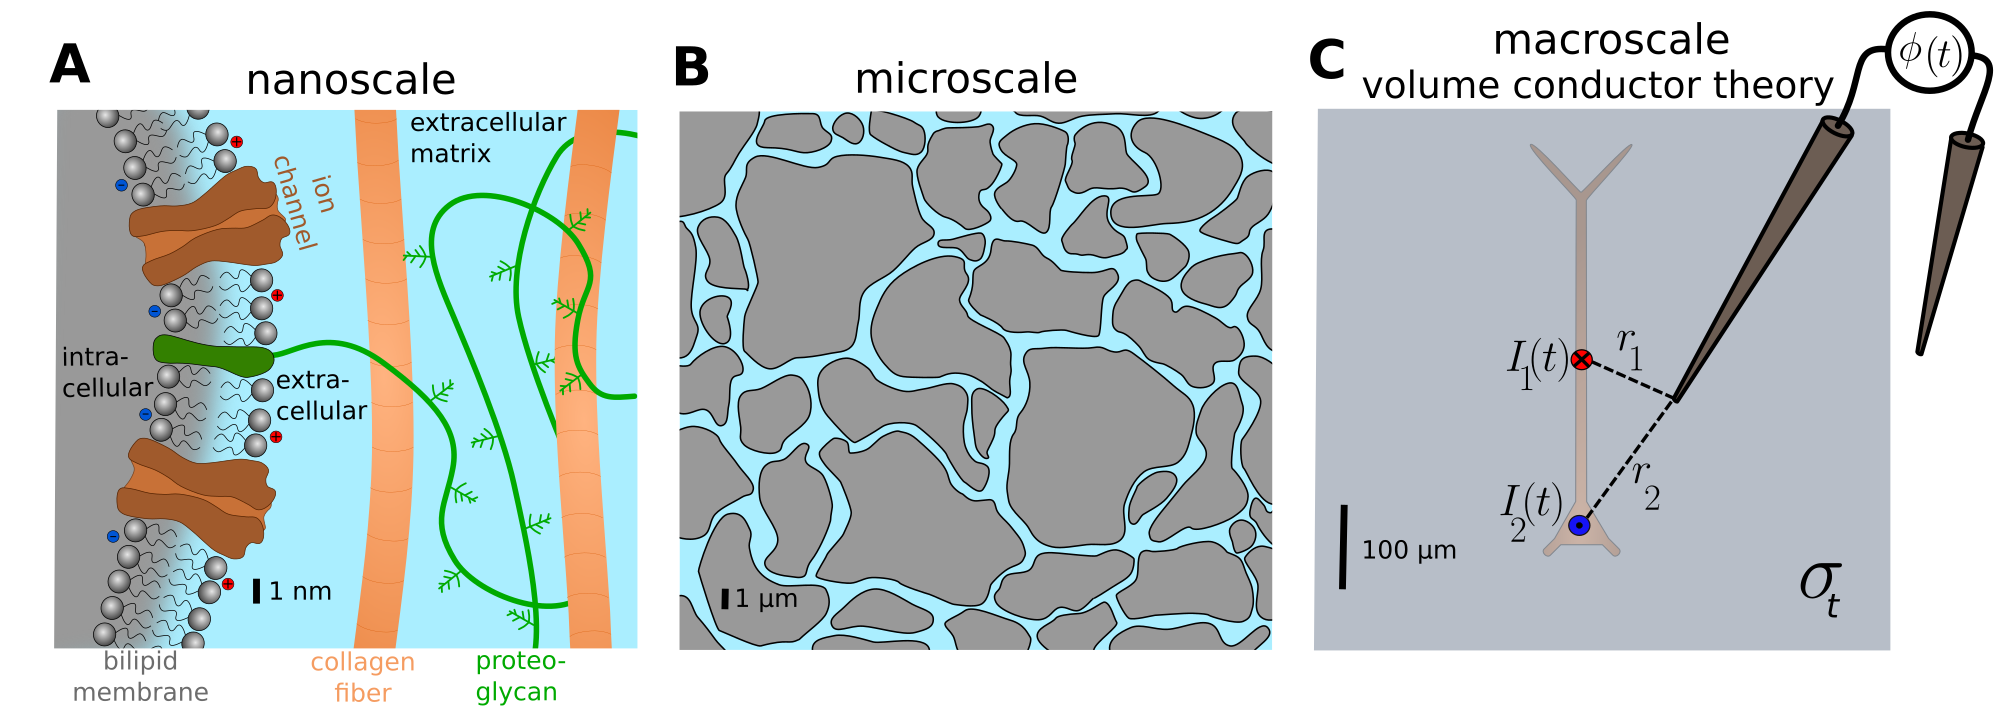
\includegraphics[width=0.8\textwidth]{Figures/VC/ecs_scales_three_levels.png}
\end{center}
\caption{\textbf{Extracellular medium at different scales}
Panel C is the level where we apply VC theory
\tvnnote{Burde denne figuren flyttes til Basics? Det er naa der vi tar mesteparten av denne diskusjonen.}
}
\label{fig:VC:ECS_scales_3levels}
\end{figure}

%%%%%%%%%%%%%%%%%%%%%%%%%%%%%%%%
\section{\blue{From neuronal current sources to extracellular potentials}}
\label{sec:VC:main}
%%%%%%%%%%%%%%%%%%%%%%%%%%%%%%%%
Throughout this chapter we shall assume that we know the neuronal transmembrane currents at all points in space. If they stem from a simulation of a multicompartmental neuron model, they are typically represented as a set of discrete current sources, i.e., one source per neuronal segment (\fref{fig:VC:CSD}{\bf A}).



As indicated above, the variables ${\bf i_t}$, $\sigma_t$ and $\phi$ can in general be functions of both position and time. However, for the remainder of this chapter, we shall for simplicity assume that $\sigma_t$ is constant. Furthermore, it is implicit in \fref{eq:VC:CSD2} that the relationship between current sources and extracellular potentials is instantaneous (i.e., we can solve \fref{eq:VC:CSD2} at each time point independently), and in the remainder of the chapter we therefore only use the positional argument for ${\bf i_t}$ and $\phi$.

In the following subsections, we show how VC-theory is used to compute $\phi$ in some idealized cases with a homogeneous extracellular medium, and then discuss how this theory can be expanded to more complex cases accounting for inhomogeneities.


%%%%%%%%%%%%%%%%%%%%%%%%%%%%%%%%
\section{\blue{Infinite isotropic homogeneous extracellular medium}}
\label{sec:VC:isohomo}
\index{Conductivity!Homogeneous and isotropic}
%%%%%%%%%%%%%%%%%%%%%%%%%%%%%%%%

We start by deriving an expression for the extracellular potential $\phi$ in the case where the extracellular medium is infinite, isotropic and homogeneous. By homogeneous we mean that the conductivity $\sigma_t$ is the same everywhere in space, and by isotropic we mean that $\sigma_t$ is the same in all spatial directions. Although the extracellular medium in reality is neither infinite, nor strictly isotropic and homogeneous, this approximation may still in many cases give fairly good predictions of $\phi$.


%%%%%%%%%%%%%%%%%%%%%%%%%%%%%%%%
\subsection{\blue{Point source approximation}}
\label{sec:VC:pointsource}
\index{Point source approximation}

%%%%%%%%%%%%%%%%%%%%%%%%%%%%%%%%
We start by deriving the contribution to $\phi$ from a single neuronal point source $I_k$ at the point ${\bf r_k}=0$ (\fref{fig:VC:pointsource}{\bf A}).

\begin{figure}[!ht]
\begin{center}
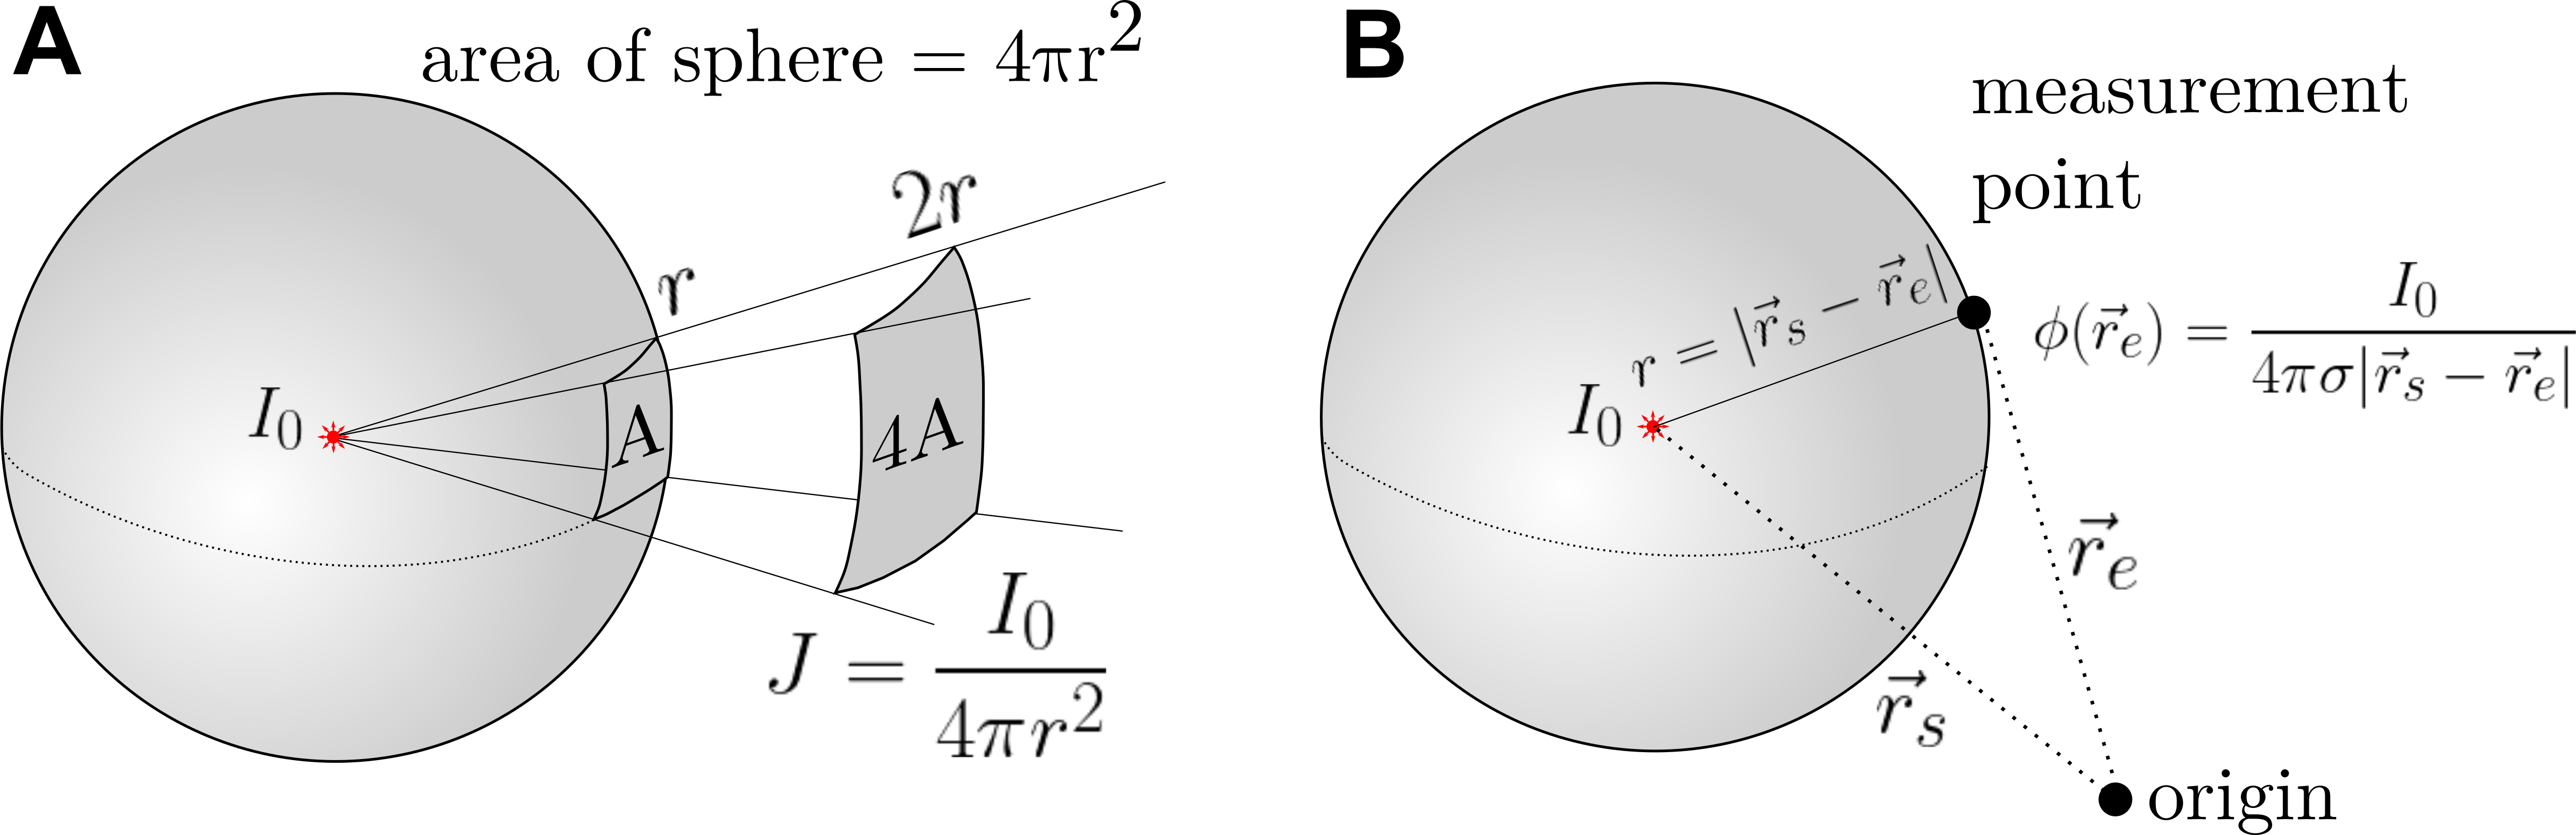
\includegraphics[width=0.8\textwidth]{Figures/VC/EP_from_pointsource_illustration.png}
\end{center}
\caption{\textbf{Extracellular potential from single neuronal point source current.}
\tvnnote{Har laget utkast til figur. Noe slikt? } \ghnote{Praktfull, men trenger index $t$ paa $\sigma_t$, og $i_t$ erstatter J.}
}
\label{fig:VC:pointsource}
\end{figure}
\snnote{Dere har kanskje diskutert dette allerede..men jeg tenker at det kanskje ikke er nodvendig aa henvise til Poisson her, siden den ikke er introdusert ennaa?}
\sntxt{\sout{Here, we could compute $\phi$ by solving \fref{eq:VC:CSD3}. However, due to the spherical symmetry of this simple case, we can take a shorter path by realizing that the current density (\fref{eq:VC:ohmici}) must} In this simple case, we know that the current density is} radially directed, and that its magnitude must be solely a function of distance $r$ from the source:


\begin{equation}
i_t({\bf r}) = i_t(r) = -\sigma_t \frac{d\phi(r)}{dr}.
\end{equation}

\snnote{Setningen under var ganske lang..hva med:}
\sntxt{\sout{Knowing this, we may find $\phi$ by simply noting that, s} S}ince there can be no charge accumulation anywhere inside the sphere, the net current $I_k$ injected into the center of the spherical volume with radius $r$ must equal the net current leaving through the surface of the volume \sntxt{.\sout{, which} The net current escaping the surface can in turn be found by multiplying \sout{in turn must equal}} the current density $i_t(r)$ at the surface \sntxt{\sout{multiplied}} with the surface area $4\pi r^2$. We then get the relationship:

\begin{equation}
I_k = -4\pi \sigma_t r^2  \frac{d\phi(r)}{dr} \, \iff \, \frac{d\phi(r)}{dr} = -\frac{I_k}{4\pi \sigma_t r^2 }.
\label{eq:VC:knut}
\end{equation}
\snnote{Hva tenker dere om aa enten sette en minus foran begge sider av 4.4 eller enda enklere bare integrere fra uendelig til r isteden? Da hadde leseren sluppet aa gange med -1 selv..}
To obtain the final solution for $\phi$, we integrate eq. \ref{eq:VC:knut} from $r$ to $\infty$:
\snnote{Forslag: (original kommentert ut)}

%\begin{equation}
%\int_r^{\infty} \frac{d\phi(r')}{dr'} dr' = \int_r^{\infty} -\frac{I_k}{4\pi \sigma_t r'^2 } dr'.
%\label{eq:VC:knut2}
%\end{equation}

\sntxt{
\begin{equation}
\int_{\infty}^r \frac{d\phi(r')}{dr'} dr' = \int_{\infty}^r -\frac{I_k}{4\pi \sigma_t r'^2 } dr'.
\label{eq:VC:knut2}
\end{equation}
}
Since $\phi({\infty}) = 0$, this leads to the final expression:

\begin{equation}
\phi({\bf r}) = \phi(r) = \frac{I_k}{4\pi \sigma_t r},
\label{eq:VC:pointsource}
\end{equation}
where $r$ is the distance from the source.

In the \sntxt{example?} above, we made things simple by assuming that the current source was placed in the origin ${\bf r} = 0$. For a point source located in an arbitrary point ${\bf r_k} $ (\fref{fig:VC:pointsource}{\bf B})), the corresponding expression for the extracellular potential is:

\begin{equation}
\phi({\bf r}) = \frac{I_k}{4\pi \sigma_t |{\bf r-r_k}|},
\label{eq:VC:pointsource2}
\end{equation}

If we have several point-current sources, $I_{1}, I_2, I_3, ... $, in locations ${\bf r_1}, {\bf r_2}, {\bf r_3} ... $, their contributions add up linearly, and the potential in a point ${\bf r}$ is given by:

\begin{equation}
\phi({\bf r}) = \frac{I_1}{4\pi  \sigma_t {\bf |r-r_1|}} + \frac{I_2}{4\pi  \sigma_t {\bf |r-r_2|} } + \frac{I_3}{4\pi  \sigma_t {\bf |r-r_3|} } + ... = \sum_k \frac{I_k}{4\pi  \sigma_t {\bf |r-r_k|} }.
\label{eq:VC:pointsources}
\end{equation}

%%%%%%%%%%%%%%%%%%%%%%%%%%%%%%%%
\Fref{eq:VC:pointsources} is referred to as the point-source approximation \cite**{Holt1999}, since it approximates the neuron as a set of point current sources, i.e., the neuron delivers to the extracellular space a singular current source per neuronal segment, located in the segment midpoint.

%%%%%%%%%%%%%%%%%%%%%%%%%%%%%%%%
\subsection{\blue{Line source approximation}}
\label{sec:VC:linesource}
\index{Line source approximation}

A more sophisticated choice may be to assume that the transmembrane current is evenly distributed over the segment axis, a choice which is referred to as the line-source approximation \cite**{Holt1999,Linden2014}. The contribution to the extracellular potential from a current $I_k$ in a segment $k$ can be found analytically by integrating \fref{eq:VC:pointsource} over the center-line axis of the compartment (see Appendix \ref{app:linesource} or \citeasnoun**{Holt1998}). For a segment with length $\Delta s_k$, the contribution to the extracellular potential will be:

\snnote{Forslag: ta bort t..}

\begin{equation}
\phi({\bf r},\sntxt{\sout{t}})_k = \frac{I_k}{4\pi \sigma_t} \int \frac{dr_k}{|{\bf r-r_k}|} =
\frac{I_k}{4\pi \sigma_t \Delta s_k} \log \left| \frac{\sqrt{h_k^2+\rho_k^2}-h_k}{\sqrt{\ell_k^2+\rho_k^2}-\ell_k} \right|.
\label{eq:VC:linesource}
\end{equation}

Here $\rho_k$ is the distance perpendicular to the line segment, $h_k$ is the longitudinal distance from the end of the segment, and $\ell_k = \delta s_k + h_k$ is the longitudinal distance from the start of the segment (\fref{fig:VC:line_source_illustration}). \Fref{eq:VC:linesource} and \fref{eq:VC:pointsource} are the equivalent expressions where the transmembrane currents in a single neuronal segment are treated as a line source and point source, respectively. As for the point-source approximation, the contributions from several line-sources add up linearly. That is, if we have multiple segments $k$, the extracellular potential can be computed as:

\begin{equation}
\phi({\bf r},\sntxt{\sout{{\bf t}}}) = \sum_k \frac{I_k}{4\pi \sigma_t \Delta s_k} \log \left| \frac{\sqrt{h_k^2+\rho_k^2}-h_k}{\sqrt{\ell_k^2+\rho_k^2}-\ell_k} \right|.
\label{eq:VC:linesources}
\end{equation}

\begin{figure}[!ht]
\begin{center}
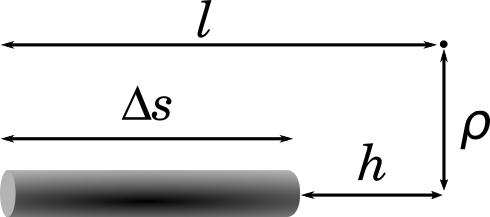
\includegraphics[width=0.5\textwidth]{Figures/VC/line_source_illustration.png}
\end{center}
\caption[]{\textbf{Line-source approximation.} Definitions of symbols used in the line-source approximation. }
\label{fig:VC:line_source_illustration}
\end{figure}

The line-source approximation can be expected to give a better prediction of $\phi$ than the point-source approximation at points in space that are very near neuronal membranes, especially when it comes to predicting rapid fluctuations in $\phi$, such as the extracellular action potential signature \cite**{Holt1999}. At points further away from membranes, the two approaches give converging predictions, see Fig.~\ref{fig:VC:point_vs_linesource}.

\begin{figure}[!ht]
\begin{center}
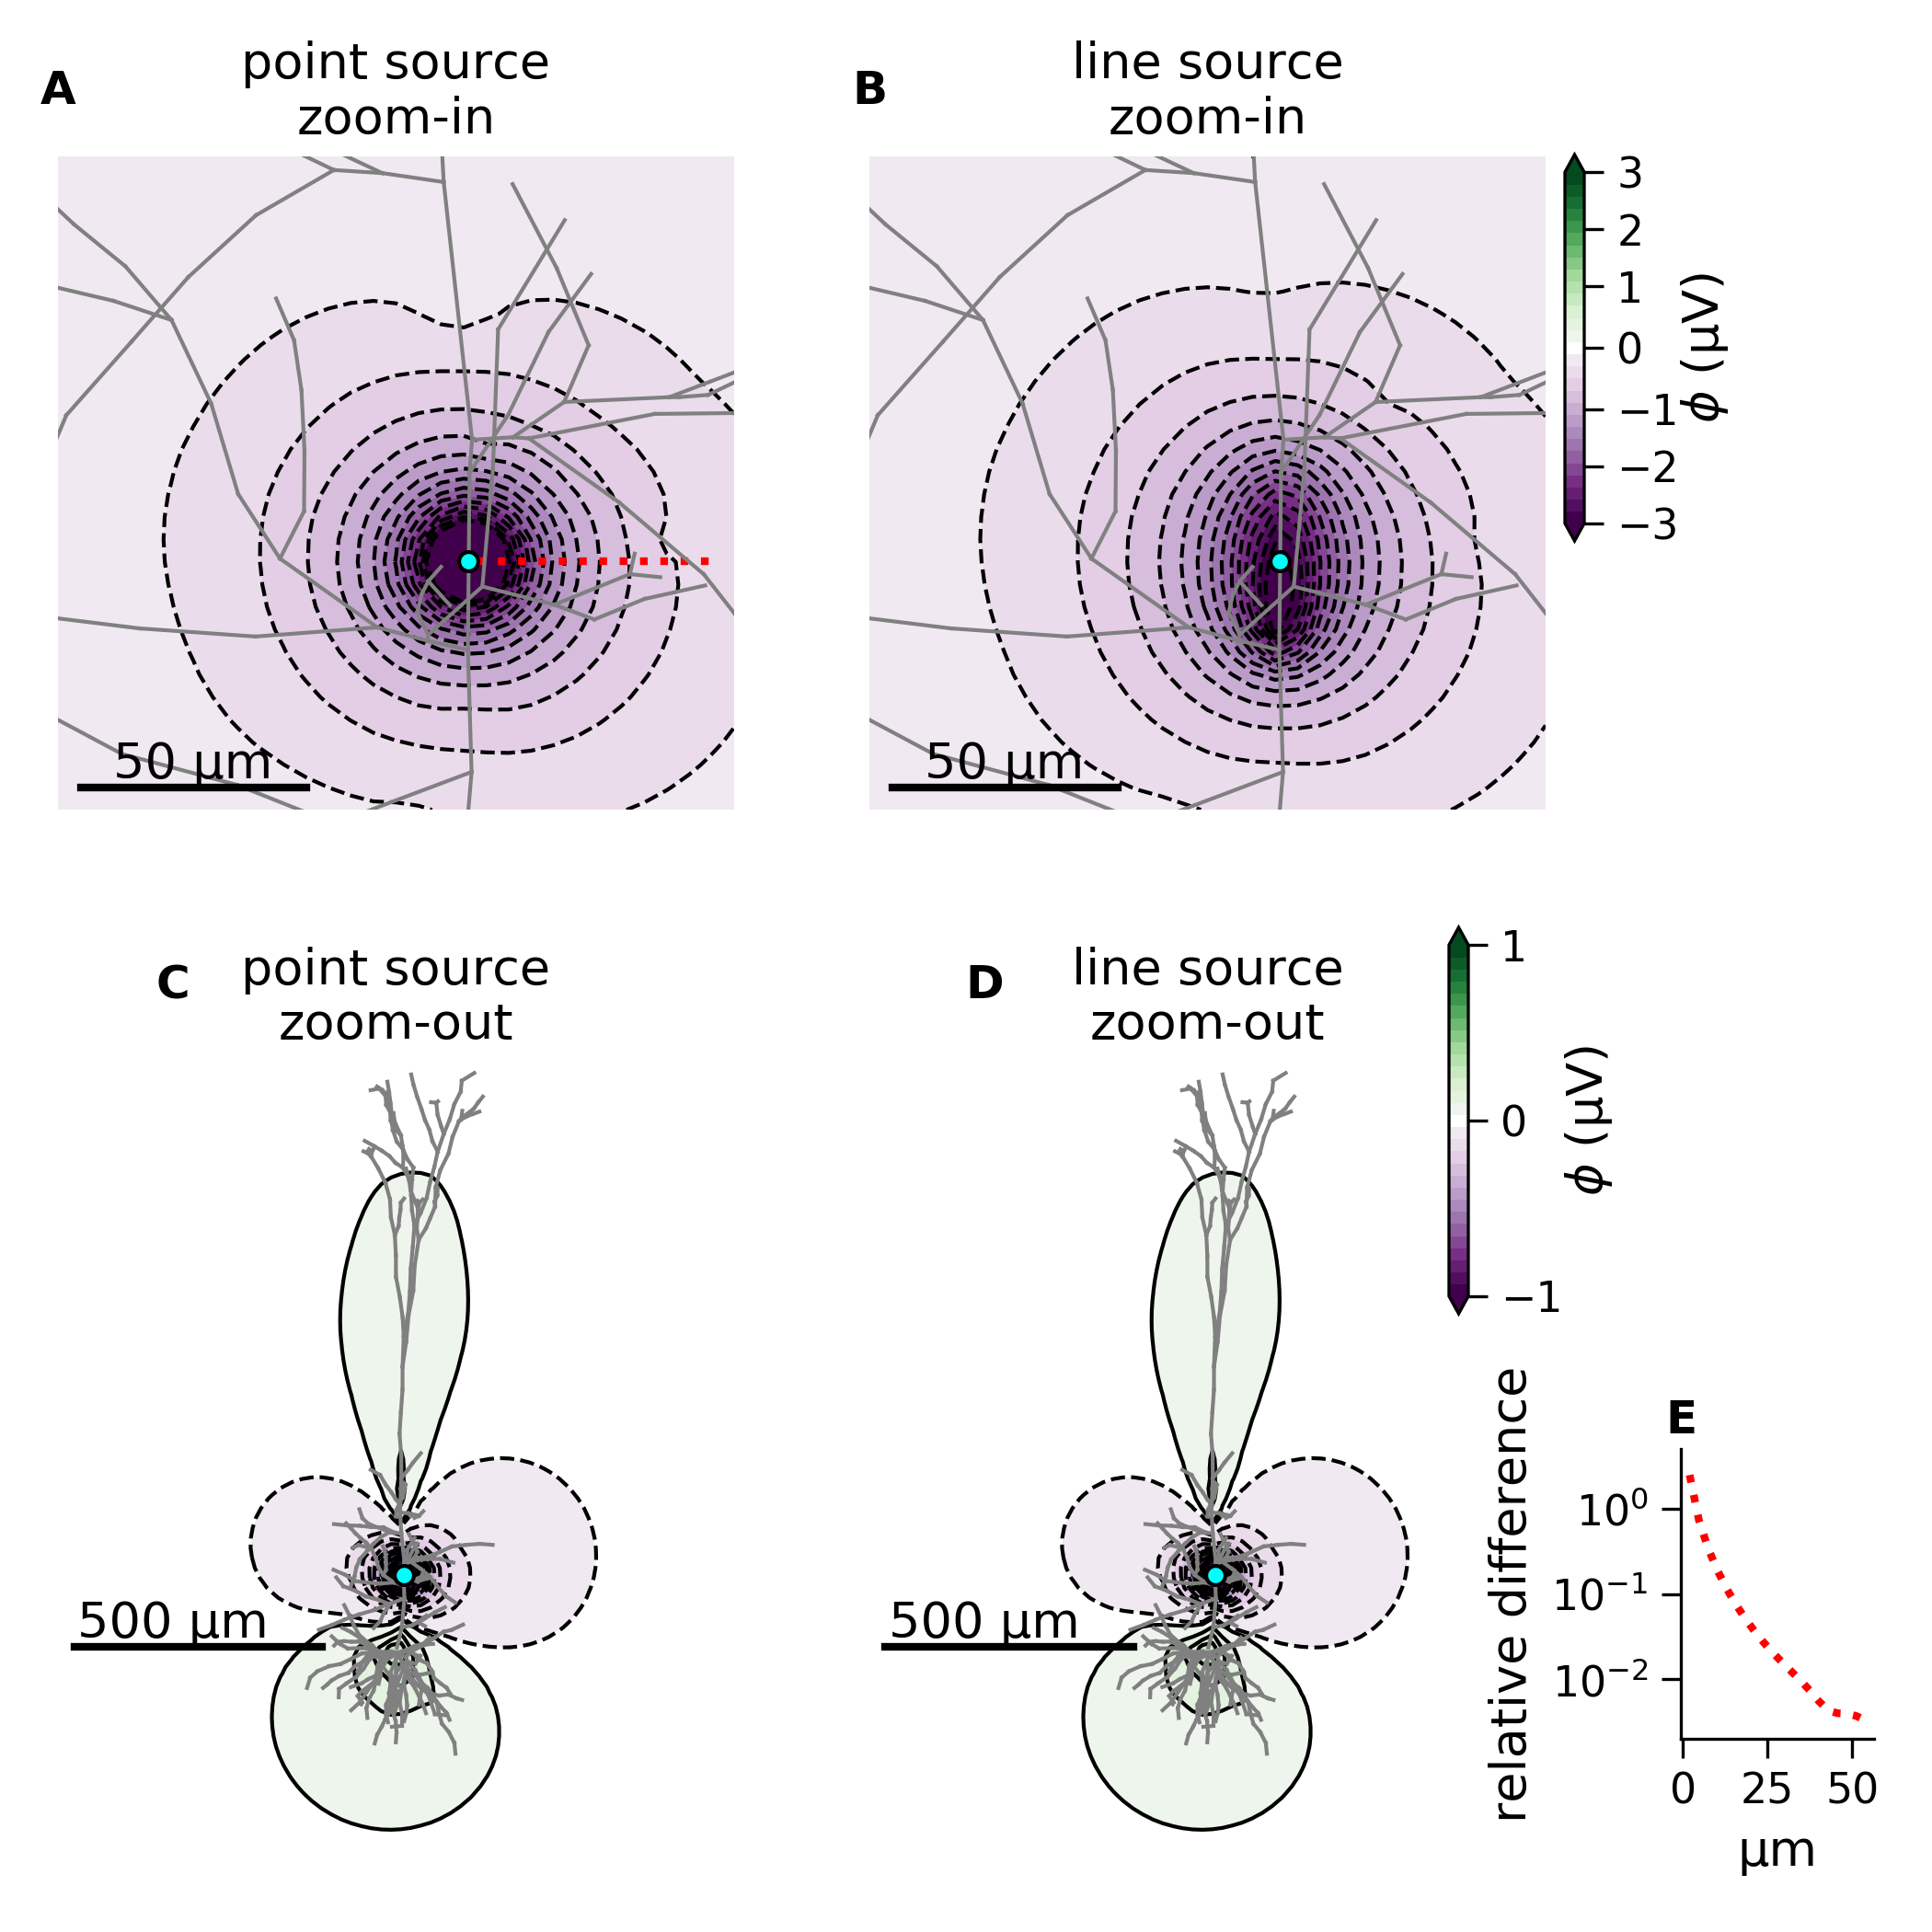
\includegraphics[width=0.7\textwidth]{Figures/VC/fig_point_versus_linesource.png}
\end{center}
\caption[]{\textbf{Point- versus line-source approximation.}
Extracellular potential at a snapshot in time following a single excitatory synaptic input (location marked by cyan dot) to a rat cortical layer 5 pyramidal neuron \cite**{Hay2011}.
The extracellular potential is shown for the time step corresponding to the maximum observed absolute value for the extracellular potential, and it is calculated from the same neural simulation, at the same time with either the point-source approximation ({\bf A}) or the line-source approximation ({\bf B}). Very close to neural current sources, the two approaches
give substantially different results, but at slightly larger differences, the results from the two approaches converge ({\bf C} versus {\bf D}). This is also illustrated in panel {\bf E}, which shows the relative difference between the results from the two approaches with increasing distance from the location of the synaptic input (red dashed line in panel {\bf A}). The relative difference was less than 10\% for distances greater than $\sim$13~\si{\micro\metre}, and less than 1\% for distances greater than $\sim$35~\si{\micro\metre}.
}
\label{fig:VC:point_vs_linesource}
\end{figure}

%%%%%%%%%%%%%%%%%%%%%%%%%%%%%%%%
\subsection{\blue{Current-source-density description}}
\label{sec:VC:CSD}
\index{Current source density}
%%%%%%%%%%%%%%%%%%%%%%%%%%%%%%%%

 As a mathematical generality, we may instead define a continuous density distribution \tvnnote{Virker litt rart for meg aa beskrive delta-funksjoner som contineous density distribution?} of current sources (\fref{fig:VC:CSD}B), which we call the \textit{current source density}\index{Current source density} (CSD), with units A/m$^3$ \tvnnote{Litt rart aa introdusere CSD her, ogsaa ikke bruke det i de foerste tilfellene. Hva med aa utsette dette til etter "line-source"?}. For example, the CSD representing the four point sources in \fref{fig:VC:CSD}A would be formulated as a sum of four delta functions.

\begin{figure}[!ht]
\begin{center}
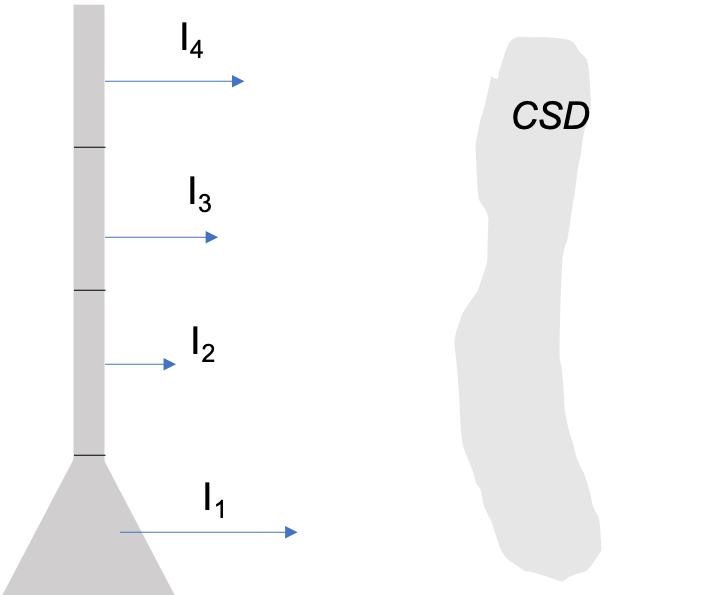
\includegraphics[width=0.5\textwidth]{Figures/VC/CSD.png}
\end{center}
\caption{\textbf{Neuronal current sources.}  {\bf (A)} When simulated on a numerical scheme, the transmembrane currents are known at a discrete set of neuronal segments, i.e., as a set of point sources.  {\bf (B)} As a mathematical generality, we can describe the transmembrane currents as a current source density (CSD) distribution, $C({\bf r},t)$. We note the sum of current entering/leaving a neuron is always zero, so that in {\bf (A)}, we must have that $I_1 + I_2 + I_3 + I_4 + I_5= 0$, and in {\bf (B)} we have that the spatial integral over $C({\bf r},t)$ must be zero at all times.
}
\label{fig:VC:CSD}
\end{figure}
Volume conductor theory is essentially based on current continuity in the extracellular medium, i.e., the requirement that no net current can enter/leave a given point\tvnnote{"Point" har jo i prinsippet ikke noen utstrekning. Kan vi bruke "volume"?}
\tvnnote{Dette gjelder kun untenfor sinks/sources da. Nevne det?} in space. Mathematically, current continuity implies that:
\snnote{Kanskje vi like gjerne kan glemme tid her?}
\begin{equation}
\nabla \cdot {\bf i_t}({\bf r}\sntxt{\sout{, t}}) = - C({\bf r}, \sntxt{\sout{t}}),
\label{eq:VC:CSD1}
\end{equation}
which is the same as we postulated previously in \fref{eq:Basics:continuity1}. Here, ${\bf i_t}$ is the extracellular current density through the brain tissue, and $C$ is the current source density. What  \fref{eq:VC:CSD1} essentially tells us, is that if a neuron outputs a current into a (infinitesimal) volume of space (the $C$ term), an equally large current leaves that volume as an extracellular current (the $\nabla \cdot {\bf i_t}$ term).

In this chapter, we shall assume that the extracellular current density is described by Ohm's law ( \fref{eq:VC:ohmici}). If we combine \fref{eq:VC:ohmici} and \fref{eq:VC:CSD1}, we get:

\begin{equation}
\nabla \left( \sigma_t({\bf r}\sntxt{\sout{, t}}) \nabla \phi({\bf r}, t) \right) = - C({\bf r}\sntxt{\sout{, t}}),
\label{eq:VC:CSD2}
\end{equation}

which simplifies to the more commonly used relation:
\begin{equation}
\sigma \nabla^2\phi({\bf r}\sntxt{\sout{, t}}) = - C({\bf r}\sntxt{\sout{, t}}),
\label{eq:VC:CSD3}
\end{equation}
in the less general case where the conductivity $\sigma_t$ is constant. Hence, if we know the distribution of neuronal current sources, we can integrate \fref{eq:VC:CSD2} or \fref{eq:VC:CSD3} to predict the electrical potential in the extracellular space surrounding the sources.

The forward modeling formulas in \fref{eq:VC:pointsources} and \fref{eq:VC:linesources} can be expressed more generally in terms of the CSD. The starting point is then \fref{eq:VC:CSD3}, which for a homogeneous and isotopic medium can be written:

\begin{equation}
\nabla^2 \phi({\bf r}) = - \frac{C({\bf r})}{\sigma_t}
\label{eq:VC:CSD4}
\end{equation}

Since this is a linear differential equation, we may solve it by first finding its Green's function, i.e., the solution to an impulse response $C({\bf r}) = I' \delta^3({\bf r-r'})$,
\ehnote{lite fan av notasjon med $'$, siden dette oftest brukes om den deriverte.}
where $\delta^3({\bf r})$ is the Dirac delta function in three dimensions, and $I'$ is the current source at this location. The general solution can then be expressed as a convolution over such Green's functions. Thus, we first seek the solution to:

\begin{equation}
\nabla^2 \phi({\bf r}) = - \frac{I' \delta^3({\bf r-r'})}{\sigma_t}.
\label{eq:VC:CSD5}
\end{equation}

We already listed the solution to this in \fref{eq:VC:pointsource2}, but we here provide a more rigorous derivation. We start by integrating both sides of \fref{eq:VC:CSD5} over an arbitrary 3D volume containing the source:

\begin{equation}
\iiint_V \nabla^2\phi({\bf r}) \,dV =  - \frac{I'}{\sigma_t} \iiint_V \ \delta^3({\bf r-r'}) \, dV,
\label{eq:VC:marit}
\end{equation}

By the definition of the delta-function, the right hand side of \fref{eq:VC:marit} is simply $I'/\sigma$. Using Gauss' theorem, we can convert the volume integral on the left hand side of \fref{eq:VC:marit} to a surface integral, so that \fref{eq:VC:marit} becomes:

\begin{equation}
\oiint_{S} \nabla\phi({\bf r}) \cdot \, d{\bf S}  = - \frac{I'}{\sigma_t},
\label{eq:VC:berit1}
\end{equation}

To solve this, it is convenient to chose the volume that we integrate over to be a sphere centered at the source location ${\bf r'}$, and with radius $R = |{\bf r-r'}|$ (\fref{fig:VC:pointsource}{\bf B}). Due to the symmetry of problem, we then know that the electrical potential is the same for all ${\bf r}$ on the surface of the sphere, so that $\phi({\bf r}) = \phi(R)$. We also know that its gradient $\nabla\phi({\bf r}) = d\phi(R)/dR$ is constant over the surface, and perpendicular to the surface increment $d{\bf S}$. If we use this, \fref{eq:VC:berit1} becomes:
\begin{equation}
\oiint_{S} \frac{d\phi(R)}{dR} d{S}  = - \frac{I'}{\sigma_t},
\label{eq:VC:berit1ogenhalv}
\end{equation}
which has the solution:
\begin{equation}
4\pi R^2 \frac{d\phi(R)}{dR} = \frac{I'}{\sigma_t}
\label{eq:VC:berit2}
\end{equation}
If we integrate this from $R$ to $\infty$, and use that $\phi(\infty) = 0$, we get:
\begin{equation}
\phi(R) = \phi({\bf r}) = \frac{I'}{4\pi \sigma_t R}.
\label{eq:VC:berit3}
\end{equation}
We may now insert back for $\phi(R)= \phi({\bf r})$ and $R = |{\bf r-r'}|$ to obtain the desired Green's function:

\begin{equation}
\phi({\bf r})= \frac{I'}{4\pi \sigma_t |{\bf r-r'}|},
\label{eq:VC:berit4}
\end{equation}
As earlier stated, the solution for a general CSD can be expressed as a convolution over the Green's function, so that:

\begin{equation}
\phi({\bf r}) = \frac{1}{4\pi \sigma_t}\iiint_V \frac{C({\bf r'})}{|{\bf r}-{\bf r'}|} \,dV,
\label{eq:VC:csds}
\end{equation}
where the volume integral runs over all sources. Here, $C$ represents whatever approximation one used for the current sources, and \fref{eq:VC:csds} is the continuous counterpart to \fref{eq:VC:pointsources}. If we describe the CSD as a sum of point sources, i.e.,  $C({\bf r}) = \sum_k I_k \delta^3({\bf r} - {\bf r_k})$,  \fref{eq:VC:csds} reduces to \fref{eq:VC:pointsources}.


\subsubsection{\blue{Derivation of the CSD equation}}
\label{sec:VC:C2}
\index{Current source density}

\tvnnote{Flyttet avsnittetet under fra Basics-kapittelet}
When we study processes on the level of brain tissue, %we often wish to work on an even coarser spatial scale\tvnnote{Litt uklart hva "even coarser" henviser til. Tidligere er jo bare skrevet mye stoerre enn nm som jo kan vaere km.}
we are typically interested in volumes $\gg 1 \, \si{\cubic\micro\metre}$. The diameter of a neural dendrites is typically $\sim 1 \,\si{\micro\metre}$, which means that the averaging volume encloses components of multiple neurites, and includes both intra- and extracellular spaces. The advantage with such a \textit{coarse-grained}\index{Coarse-grained} resolution, is that both cellular and extracellular currents will be defined over the whole tissue-space, rather than within their respective sub-spaces \cite**{Gratiy2017}. At this spatial scale, the intracellular current, for example, does not \tvntxt{necessarily} interpret as belonging to a specific neuron, but rather as the average intracellular current within the whole volume, containing contributions from several different neurons. Likewise, also the transmembrane currents and extracellular currents are volume averages. 
\tvnnote{Litt usikker paa dette. For meg er alltid transmembrane stroemmer knyttet til ett nevron. Boer spesifiseres mer, eller taes bort?}
\gen{Kanskje vi kunne hatt en liten figur som viser de tre skalaene vaare (atom, cell ("concentration"), tissue)? Egentlig er vel 
nanometer (10 i minus 9), micrometer (10 i minus 6) og millimeter (10 i minus 3) ganske typiske lengder for disse tre skalaene selv om tissue jo kan vaere stoerre enn en millimeter.}


Although \fref{eq:Basics:continuity1} may seem intuitively reasonable, we introduced it above more or less as a postulate. A thorough derivation of this equation was given by \citeasnoun**{Gratiy2017}, and for the interested reader, we will here go through the main steps of this derivation. 

In general, current conservation implies that: 
\begin{equation}
{\bf \nabla} \cdot {\bf i}_\text{tot} = 0, 
\label{eq:Basics:Sergey1}
\end{equation}
where we can think of ${\bf i}_\text{tot}$ as the total current density defined on the relatively fine spatial scale where it is meaningful to distinguish between it being either cellular or extracellular. Let us further define $\left<{\bf i}_\text{tot}\right>$ as being this total current when averaged over some coarse-grained volume that spans over both intra- and extracellular spaces. 
As current conservation also applies at this scale \gen{Kanskje det kan forklares med en setning? MEMBRANSPALTING?}, we have that: 
\begin{equation}
{\bf \nabla} \cdot \langle{\bf i}_\text{tot}\rangle = 0.
\label{eq:Basics:Sergey2}
\end{equation}
Since we may perform the averaging separately over the cellular (c) \gex{(Inkluderer "cellular" baade  "intracellular" og membranen?)} and extracellular (e) domains, we have that $\langle{\bf i}_\text{tot}\rangle = \langle{\bf i}_\text{tot}\rangle_\text{c} + \langle{\bf i}_\text{tot}\rangle_\text{e}$. With this, we can may write \fref{eq:Basics:Sergey2} as:
\begin{equation}
{\bf \nabla} \cdot \langle{\bf i}_\text{tot}\rangle_\text{c}  + {\bf \nabla}\cdot \langle{\bf i}_\text{tot}\rangle_\text{e} = 0
\label{eq:Basics:Sergey3}
\end{equation}
In Appendix A of \citeasnoun**{Gratiy2017}) it was shown that the divergence of the coarse-grained current density over the cellular domain can be expressed as a sum of transmembrane currents (i.e., as the CSD term ($C$) that we introduced in \fref{eq:Basics:continuity1}. Further, if we rename the average current running extracellularly through tissue $\langle{\bf i}_\text{tot}\rangle_\text{e}$ to ${\bf i}_\text{t}$, we see that \fref{eq:Basics:Sergey3} becomes identical to  \fref{eq:Basics:continuity1}. 

The derivation of \fref{eq:Basics:continuity1} thus reveals that it only has a meaningful interpretation when considering tissue in a coarse-grained scale, i.e., a spatial scale large enough to contain both intra- and extracellular domains.\tvnnote{Er dette noedvendigvis sant? Ligningen i seg selv er vel ganske generell og blir jo brukt i EMI (Tveito) osv, og boer vel kunne loeses nummerisk paa micrometer nivaa?}
Importantly, ${\bf i}_\text{t}$ thus interprets as the average current running extracellularly through tissue, defined as extracellular current per unit \textit{tissue} cross section area and not per \textit{extracellular} cross section area (although it only runs through the extracellular parts of this cross section area). Similarly, $\sigma_\text{t}$ in \fref{eq:Basics:continuity2} interprets as average conductivity experienced by the current ${\bf i}_\text{t}$. As this current will face cellular obstacles, and is restricted to run only through the extracellular parts of the tissue, $\sigma_\text{t}$ is generally lower than the conductivity of the extracellular saline solution (see \fref{chap:Sigma} for further discussion). 


%%%%%%%%%%%%%%%%%%%%%%%%%%%%%%%%
\section{\orange{SN: Dipole approximation}}
\label{sec:VC:dipole}
\ghnote{GH: Jeg skrev en skisse til dette kapittelet, men fint om SN kan gaa gjennom.}
\ehnote{Jeg ville skrevet dette ut fullt likt som under "Spherical form" paa Wikipedia https://en.wikipedia.org/wiki/Multipole\_expansion.
En annen ting er at dipol/multipolapproksimasjon ikke er en "volum-konduktor-modell" som dette kapitlet dreier seg om - kanskje det boer flyttes et anna sted}
\ghnote{GH: Det som staar paa Wiki-siden er multipolekspansjon basert paa ladninger. Vaar er basert paa stroemkilder. Premisset for vaar multipolekspansj er da VC-teori, saa jeg synes stoffet hoerer hjemme her. Vi har en mer substansiell utledning i appendix, og vi bruker stort sett metoden kun i tilfeller da vi gjoer dipol-forenklingen. Derfor synes }


%%%%%%%%%%%%%%%%%%%%%%%%%%%%%%%%
The \textit{dipole approximation} \index{Dipole approximation} is an alternative to \fref{eq:VC:pointsources} for predicting the extracellular potential. The approximation is good provided that the "measuring point" for $\phi$ is far away from the source-sink distribution that it originates from, like in the case of EEG.

To be more precise, if the distance from the center of the volume containing the current sources to the measurement point is larger than the maximal distance from volume center to any source \cite**{Jackson1998}, we can reformulate \fref{eq:VC:pointsources} by using the the multipole expansion \cite**{Nunez2006}:

\begin{equation}
\phi(R) = \frac{C_{monopole}}{R} + \frac{C_{dipole}}{R^2} + \frac{C_{quadrupole}}{R^3} + \frac{C_{octopole}}{R^4} + ...
\label{eq:VC:multipole}
\end{equation}
where $R$ is the distance from the center of the source distribution, $C_{monopole}$ is the monopolar contribution of the CSD to $\phi$, $C_{dipole}$ is the dipolar contribution from the CSD to $\phi$, and so on. The derivation of this expression can be found in Appendix \ref{app:dipoleappendix}.

As we explained in \fref{sec:Neuron:membranecurrents}, the net sum of currents over a neuronal membrane is always zero, meaning that the monopolar contribution, i.e., first term in \fref{eq:VC:multipole}, vanishes. Furthermore, the quadrupole, octopole and higher-order contributions to $\phi$ decay rapidly with distance $R$. Provided that we are sufficiently far away from the source distribution, $\phi$ can therefore be well approximated by dipole contribution alone:

\begin{equation}\label{eq:VC:CDA}
\Phi(\mathbf{R}) \approx \frac{1}{4 \pi \sigma_t} \frac{|\mathbf{p}| \cos \theta}{R^2},
\end{equation}
where we have expressed $C_{dipole}$ in terms of the current dipole moment ($\mathbf{p}$), the angle ($\theta$) between the current dipole moment and the distance vector ($\mathbf{R}$), as explained in Appendix \ref{app:dipoleappendix}.

The current dipole moment is a function of the sum of all the transmembrane currents in a neuron \cite**{Pettersen2008,Pettersen2014,Nunez2006}:
\begin{equation}
\mathbf{p} = \sum_{k=1}^N I_k \mathbf{r}_k.
\label{eq:VC:dipole}
\end{equation}
For example, if we have a simple two-compartmental (and purely dipolar) neuron with a current sink $-I$ at location $\mathbf{r}_1$ and a current source $I$ at location $\mathbf{r}_2$, the current dipole moment can be formulated as $\mathbf{p} = -I\mathbf{r}_1 + I\mathbf{r}_2 = I(\mathbf{r}_2 - \mathbf{r}_1) = I\mathbf{d}$. Here $\mathbf{d}$ is the distance vector between the current sink and the current source, giving the length $d$ and direction of the current dipole.

As we mentioned above, the current dipole approximation is only applicable when we are at some distance away from the source distribution. As a rule of thumb, the approximation is thought to be good when $R$ is three to four times greater than the dipole length: $R > 3d$ or $R > 4d$ \cite**{Nunez2006}. It has been found to work well for predicting the extracranial EEG signal, but less well for intracranial electrocorticography (ECoG) \cite**{Naess2020}.


\section{\blue{Modeling recording electrodes}}
\label{sec:VC:electrodes}
\index{Electrode model}
\tvnnote{Paa sikt vil jeg gjerne spoerre noen elektrode-folk vi kjenner om aa kontroll-lese denne seksjonen, for eksempel Martinsen, Nelson, Frey eller Obien.}
%\gen{Kanskje det kunne vaere en ide aa ogsaa beskrive methods-of-imaging og modellering i MEAs her?
%Hadde foerst tenkt aa ta det med i Spikes-kapitlet. Men den gjelder jo like mye for LFP og har blitt brukt av oss i denne
%sammenheng i flere prosjekter med Ness eller Pettersen som foersteforfatter.}
%\tvnnote{Jeg tenker dette passer best i naavaerende 5.3, "Non-homogeneous extracellular medium"?}

We have demonstrated how we can use VC theory to make predictions about the extracellular potentials at any point in space following some neural activity. However, in experiments these extracellular potentials must be measured through some kind of measurement electrode. The presence of such a measurement electrode might itself affect the measured potentials in several different ways, depending on both the electrode and the extracellular potential that is being measured. Here we present a short review of different approaches to model such effects.

Recording electrodes essentially consist of an electrode surface in direct contact with neural tissue, connected with a wire to an amplifier that measures the potential relative to a reference electrode \cite**{Martinsen2008}, see \fref{fig:VC:elec_circuit}{\bf A}.
To accurately measure the potential at the electrode surface, the measurement electrodes themselves must have a very low resistance so that no potential drop occurs from the measurement site to the amplifier. The electrodes are therefore typically made of a highly conductive metal like silver or platinum, and the potential directly on the inside of the electrode surface is in practice homogeneous. The amplifier must however have a very high impedance, so that a negligible amount of current will cross the tissue-electrode interface, as this can cause electrode polarization effects\index{Electrode polarization} \cite**{Schwan1992,Martinsen2008,Moulin2008,Ishai2013}. The homogeneous potential inside the recording electrode ideally corresponds to a spatial average of the potential across the outer surface of the electrode \cite**{Nelson2008,Nelson2010,Ness2015,Vermaas2020b}.
An "ideal" electrode\index{ideal electrode} is the hypothetical case where the measured potential reported by the amplifier is identical to the "true" extracellular potential at the tip of the recording electrode (with the extracellular potential unaffected by the electrode itself). In reality there are however several different complicating factors which can cause the measured potential to differ from the "true" potential \cite**{Robinson1968,Martinsen2008,Nelson2008}.

\begin{figure}[!ht]
\begin{center}
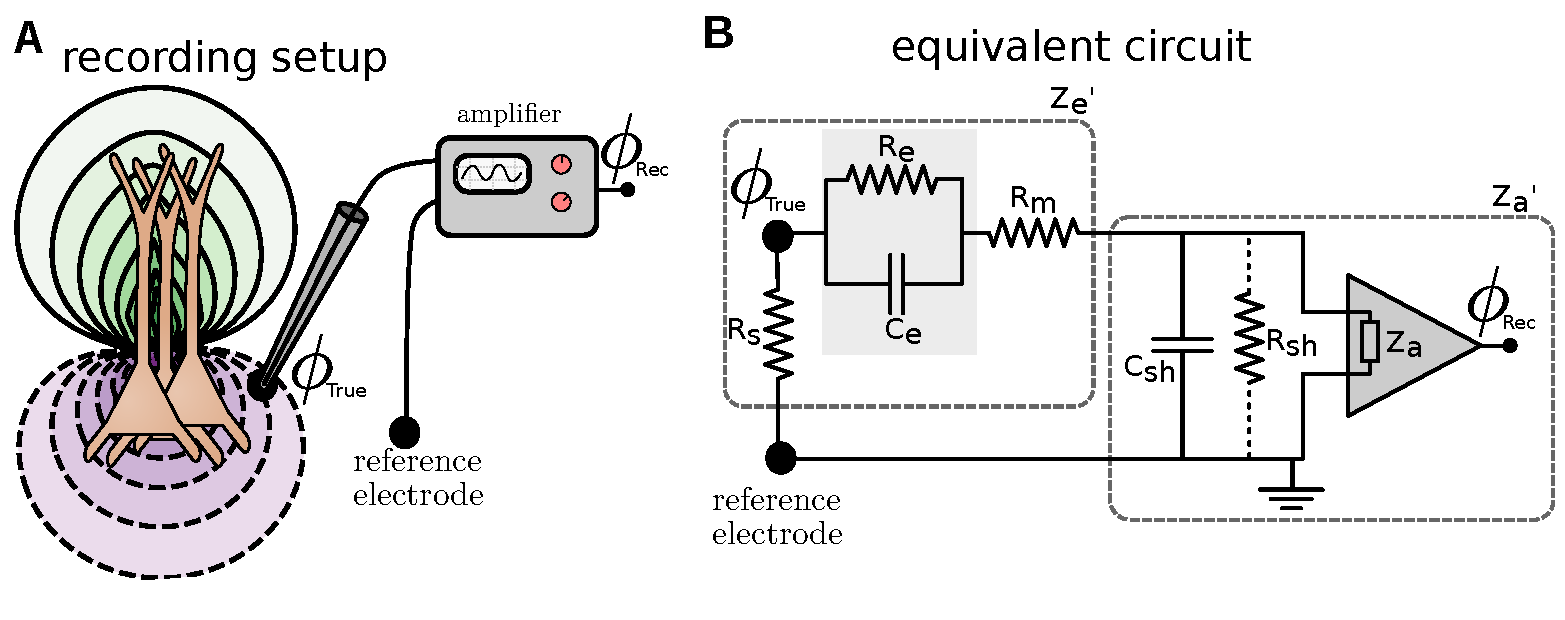
\includegraphics[width=1\textwidth]{Figures/VC/rec_elec_expanded_equivalent_circuit.pdf}
\end{center}
\caption[]{\textbf{Illustration of recording setup and equivalent circuit}
{\bf A}: The extracellular potential is measured between a recording electrode and reference electrode.
{\bf B}: An simple example of an equivalent circuit describing the recording setup, see main text and
\citeasnoun**{Robinson1968}, \citeasnoun**{Nelson2008}, \citeasnoun**{Obien2015}, and \citeasnoun**{Viswam2019}.
}
\label{fig:VC:elec_circuit}
\end{figure}

To understand and/or model such effects it is convenient to represent the recording set-up as an equivalent circuit diagram \cite**{Geddes1997}, see \fref{fig:VC:elec_circuit}{\bf B} for an example inspired by \citeasnoun**{Robinson1968}, \citeasnoun**{Nelson2008}, \citeasnoun**{Obien2015}, and \citeasnoun**{Viswam2019}.
Here $\phi_{\rm True}$ is the "true" extracellular potential at some location in the brain, caused by some neural activity, and $\phi_{\rm Rec}$ is the potential reported by the amplifier.
$R_s$ is the resistance of the extracellular medium from the measurement point to the reference electrode.
The surface of the electrode, that is, the electrode-electrolyte interface, is often modelled as a resistance, $R_e$, and a capacitance, $C_e$, in parallel (gray shaded area in \fref{fig:VC:elec_circuit}{\bf B}) \cite**{Martinsen2008,Nelson2008,CamunasMesa2013,Viswam2019}. Importantly, the values of both $R_e$ and $C_e$ are typically expected to be highly frequency dependent \cite**{Martinsen2008,Nelson2008,Viswam2019}, and are often considered to be approximately proportional to $1/\sqrt{f}$ \cite{Robinson1968}, where $f$ is the frequency (implications of this frequency dependence is discussed below).
The wire from the electrode-electrolyte interface to the amplifier has resistance $R_m$, typically assumed to be negligible.
$C_{sh}$ and $R_{sh}$ represents all the shunt capacitance and resistance to ground that occurs between the electrode surface and the amplifier, through wires, connections etc., where often $R_{sh}$ is assumed to be negligible.
Finally, $Z_a$ is the amplifier input impedance.

Two important concepts here are the effective electrode impedance, $Z_e'$, and the effective amplifier input impedance, $Z_a'$. Here, $Z_e'$ is the combined impedance of the extracellular medium ($R_s$), the electrode-electrolyte interface ($R_e$, $C_e$) and the metal wire ($R_m$), while $Z_a'$ is the total impedance to ground from after the metal wire, which includes the shunt current and the amplifier itself (\fref{fig:VC:elec_circuit}{\bf B}).
For the recorded potential, $\phi_{\rm Rec}$ to be as similar as possible to the true potential, $\phi_{\rm True}$,  it is vital that $Z_a' \gg Z_e'$. If this is not fulfilled,
the recorded potential will have frequency-dependent phase- and amplitude distortions \cite**{Nelson2008,Nelson2010,Obien2015,Viswam2019}.
Importantly, the effective electrode impedance, $Z_e'$, increases strongly for low frequencies and is typically much more frequency dependent than the effective amplifier input impedance, $Z_a'$ \cite**{Nelson2008}. This means that some given recording equipment might be able to measure extracellular spikes with negligible distortion, while at the same time substantial phase and amplitude distortions might be present in LFP signals measured by the same equipment \cite**{Nelson2008,Nelson2010,Viswam2019}.
Note that metallic recording electrodes are typically unable to measure static (DC) potentials, or capture changes slower than $\sim$ 0.1 Hz.
\gen{Hvor har vi dette tallet fra?}
\ehnote{jeg er ogsaa overrasket over at metallelektroder ikke kan maale konstante potensialforskjeller i en loesning (i all den tid det finnes frie ioner i loesningen)?}
\tvnnote{Jeg vet ikke om noen laerebok referanse, men det var det som ble oppgitt som nedre grense baade av Dirk og Anna (altsaa alle tilfeller jeg har vaert borti eksperimentell data), se Miceli-artikkelen, Uhlivora-artikkelen, og ogsaa Einevoll et al., 2007. Fra en av Anna's nyere artikler fant jeg frem til dokumentasjonen paa amplifieren de har brukt, og der staar det "Lower cutoff frequency configurable from 0.1 Hz to 500 Hz", men jeg vet ikke helt om forklaringen jeg har gitt over er helt riktig.}
\ehnote{Det er vel da mer en begrensning med sampling apparat enn selve elektrodemaalingen. Si du sampler mange kanaler med int16 presisjon - det blir da et problem hvis DC-verdiene fluktuerer mye mer enn selve signalet (e.g., LFP).}
Such DC potentials can be present in neural tissue, and can often arise in simulated extracellular potentials from cell models with active conductances, for example because of the $I_{\rm h}$-current \cite**{Ness2016}. In such cases, the simulated baseline (or mean) extracellular potential is typically subtracted from the extracellular potentials to effectively remove the unobservable DC-potential.



%\begin{figure}[!ht]
%\begin{center}
%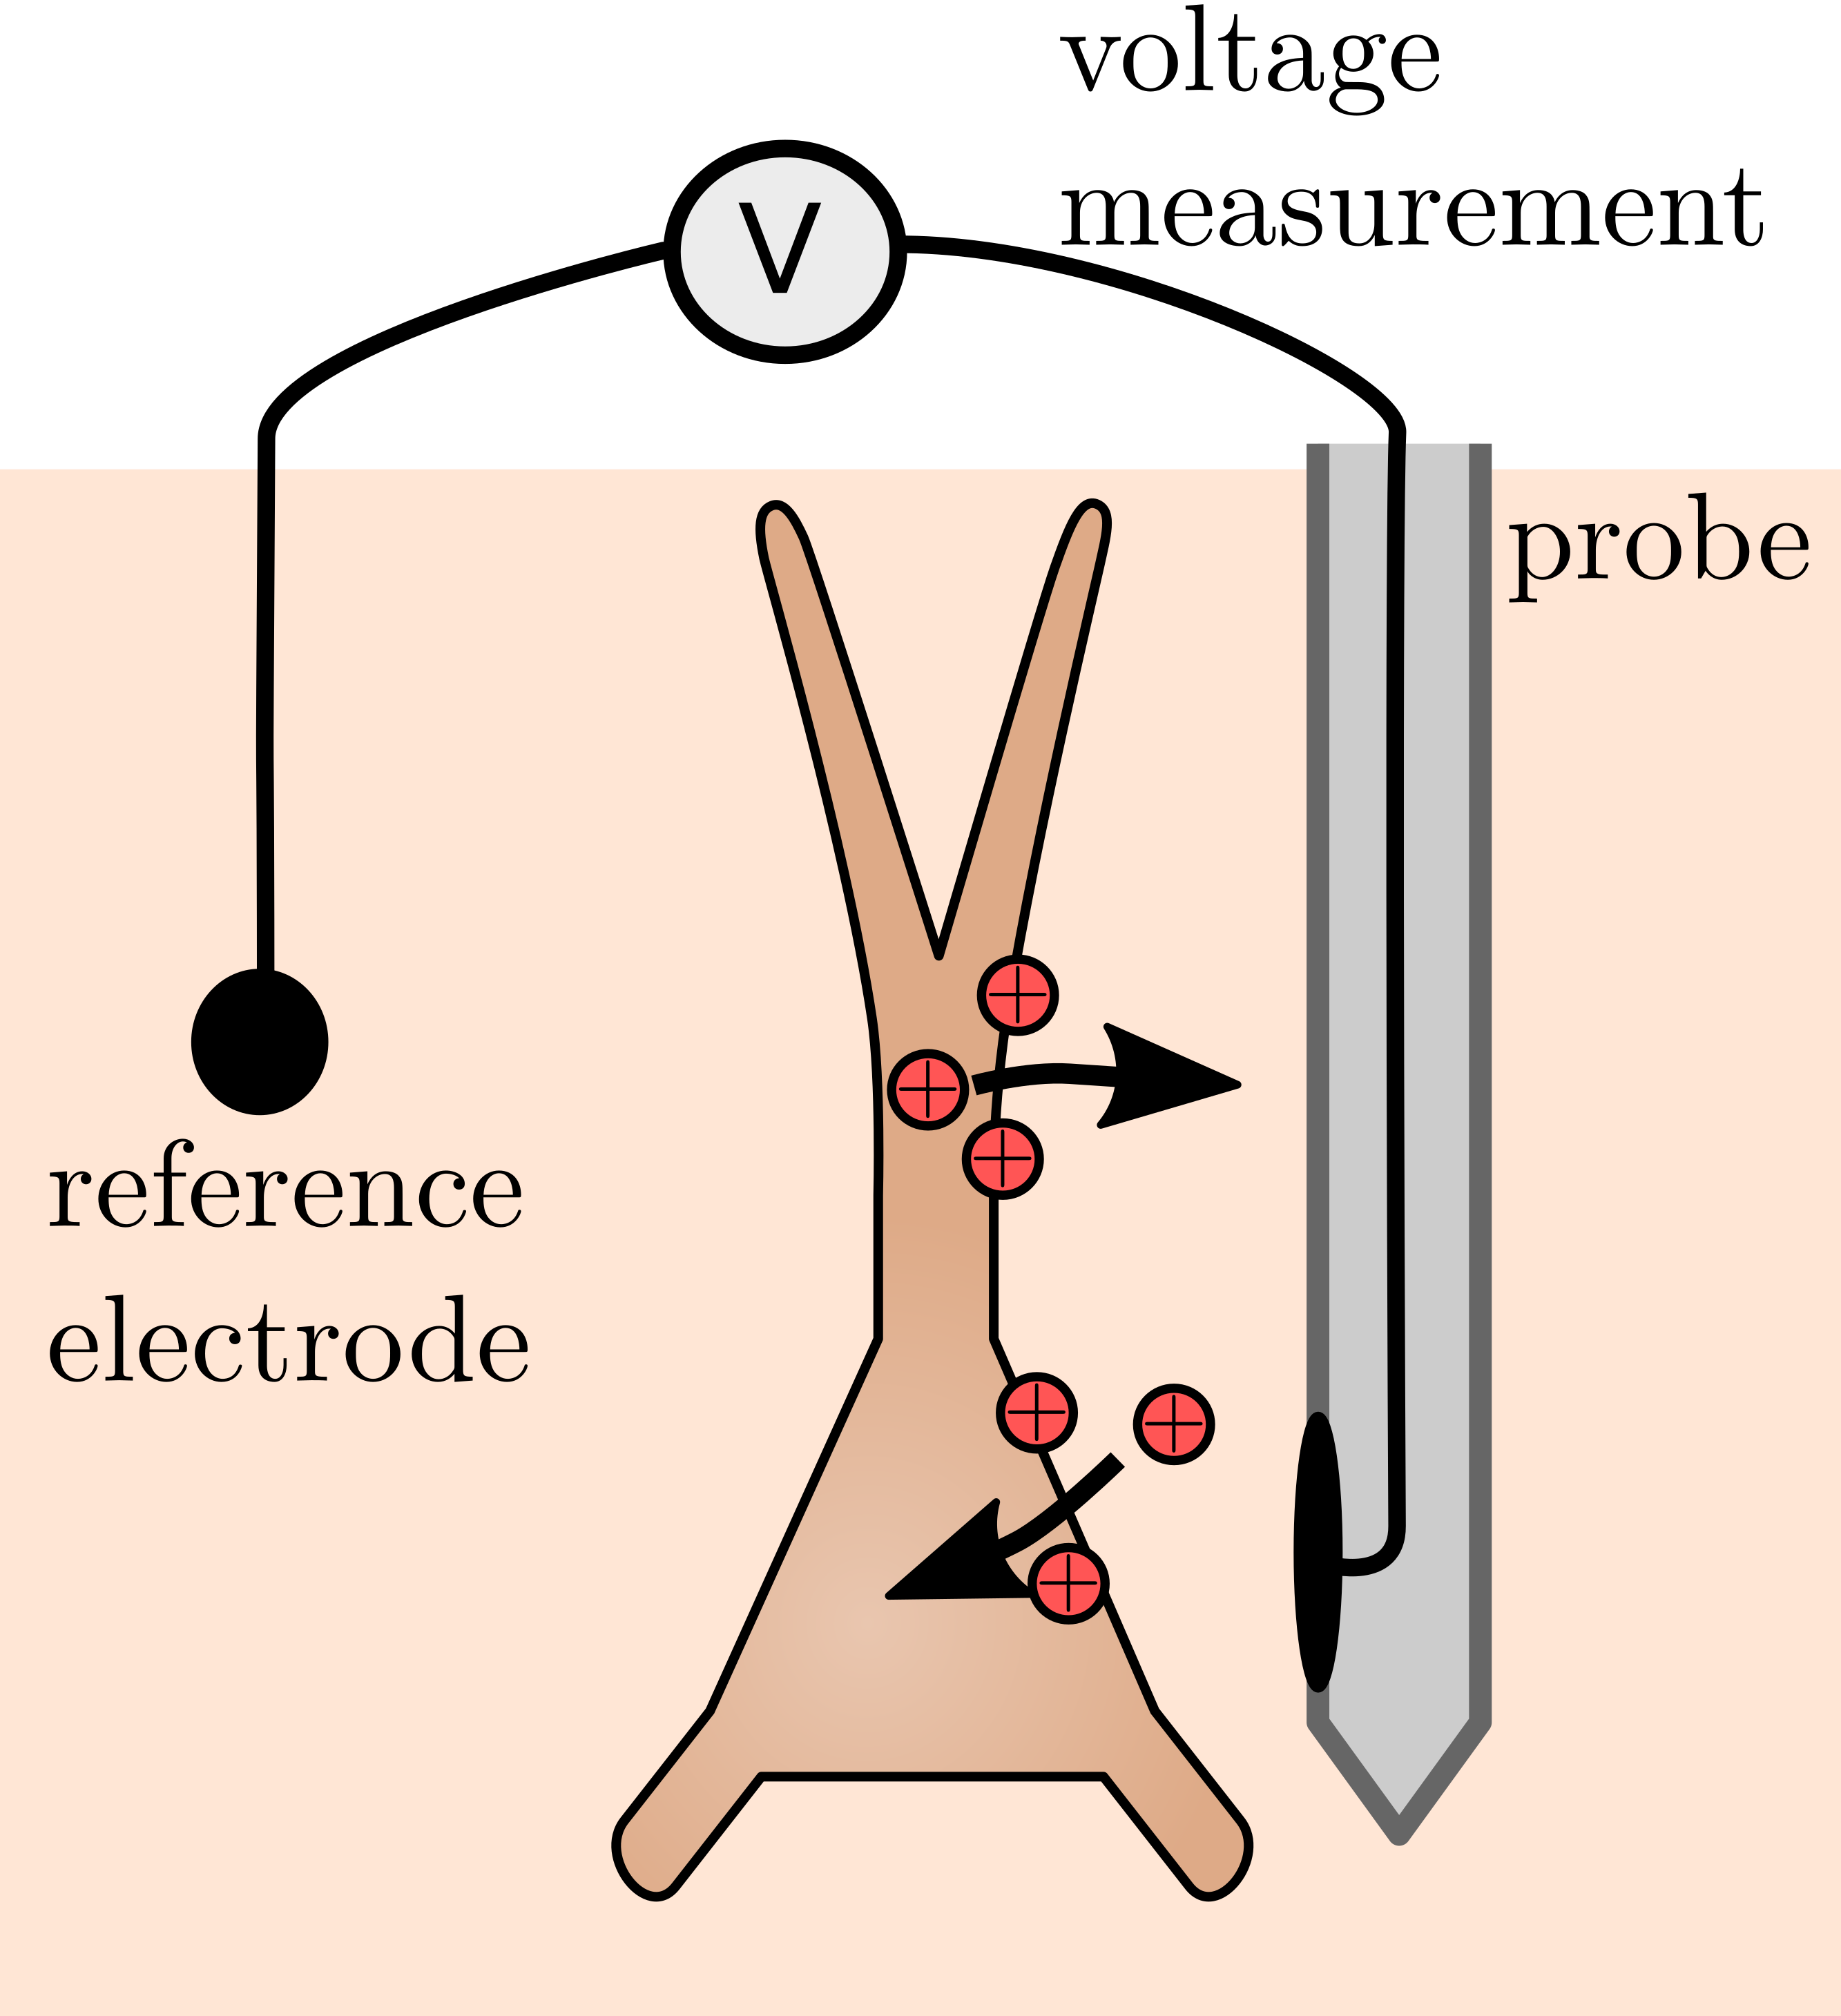
\includegraphics[width=0.4\textwidth]{Figures/VC/rec_elec_circuit.png}
%\end{center}
%\caption[]{\textbf{Illustration of recording circuit}
%Electric potential is measured between recording electrode and reference electrode, and represents the energy required to move a positive test charge from the reference electrode and to the measurement electrode. If, say, positive ions are leaving the extracellular medium (and entering a cell) in the vicinity of the recording electrode, then the energy needed to move a positive charge to the measurement electrode is negative, that is, one can gain energy by moving the charge there.  \ghnote{Litt usikker paa energi-betraktningene her. Dvs. ikke paa om de er riktige, men om de hjeper leseren...} \tvnnote{Ja, enig. Men jeg foeler det hadde vaert fint aa forklare et sted hvorfor for eksempel negatv transmembran stoem gir negativt maalt potensial. Kunne denne figuren (eller noe lignende) vaert med i for eksempel seksjon 2.3?}
%}
%\label{VC:fig:elec_circuit}
%\end{figure}

Apart from the issues discussed above, it has been convincingly argued that, provided that the proper recording equipment is used (so that $Z_a' \gg Z_e'$), electrode impedance or other electrode properties should not substantially distort recorded potentials \cite**{Martinsen2008,Moulin2008,Nelson2008,Nelson2010}.
  Note that this only applies to recording electrodes, and that substantially more complex electrode models might be needed to accurately represent current stimulation electrodes because of electrode polarization, see \fref{sec:EPI}.

Under the assumption that the proper recording equipment is used \cite**{Nelson2008,Nelson2010}, electrode properties can still affect the recorded potential.
For example, since the (homogeneous) potential directly on the inside of the electrode surface corresponds to a spatial average of the potential on the outside, the area of the electrode surface will affect over how large a region the extracellular potential is averaged over.
In practice, this means for example that extracellular action potentials (which are very spatially confined) will be less prominent on electrodes with diameters larger than $\sim$30~$\mu$m \cite**{Moffitt2005,Moulin2008,Viswam2019}, see \fref{sec:Spikes:electrode_size}.

%if the extracellular potential changes across the outer surface of the recording electrode, this can introduce a spatial filtering effect on the measured potentials.
%\gen{Her maa vi vaere presise. Potensialet paa selve elektroden vil vaere det samme, det som vil variere er hva potensialet ville vaert paa denne "virtuelle" flaten hvis det ikke hadde vaert en metallisk elektrode der.}
%In practice, this means for example that extracellular action potentials (which are very spatially confined) will be less prominent on electrodes with diameters larger than $\sim$30~$\mu$m \cite**{Moffitt2005,Moulin2008,Viswam2019}, see Section~\ref{Spikes:sec:elec_size}.

\ghnote{En eventuell diskusjon av hvor man plasserer referanseelektrodene kan inngaa her. Kommentarene under er sakset inn fra tidligere diskusjoner i Basics-kapittelet:} \tvntxt{When recording extracellular potentials in the brain, we are in principle free to arbitrarily choose the location of the reference electrode. The ideal location for the reference electrode depends on several different factors, but it is commonly placed "far away" from the neural activity that is being measured from so that the measured potential is not dependent on an unknown varying electrical activity around the reference electrode. When modelling extracellular potentials, the reference electrode is typically (and often implicitly) placed at "infinity". } \ghnote{Stemmer egentlig dette? Slik jeg forsto Sharott vil man i motsetning til det dere skriver ofte ha referanseelektroden naer maaleelektroden naar man maaler MUA, for paa den maaten aa filtrere bort effekter fra "nest naermeste nabo". Hva var galt med mitt (mer vage) forslag:} \ghtxt{When we record extracellular potentials in the brain, we can choose to place the reference electrode close or far away from the recording electrode, depending on the kind of signal one wishes to measure \cite**{Sharott2015}.} \ghnote{Kanskje si: Naar man modellerer er den i infinity. Stort sett skal vaere langt unna.} \gen{Kanskje si enda klarere at man oensker at potensialet paa referanseelektroden skal vaere saa konstant som mulig under eksperimentet (eller blir dette sirkulaert?), husker at Anna plasserte referanseelektroden i nakken paa rottene hun gjorde maalinger fra. Kanskje vi kan hoere med eksperimentalistene paa CINPLA hva de gjoer?} \ghnote{Sikkert lurt aa spoerre noen, ja, men saa vidt jeg skjoenner er dette et vanskelig spoersmaal der mange avveininger maa gjoeres.} \ghnote{Poenget er aa plassere den der det er mest praktisk - best mulig signal for det du er ute etter. }

\subsection{\blue{Point-electrode approximation}}
\label{sec:VC:point-electrode}
\index{Point-electrode}
The most straightforward and also most common approach when modeling extracellular recordings is to use the ideal point electrode approximation. This corresponds to
ignoring any potential effect from recording electrodes or electrode shanks, and calculating the extracellular potential at single points. For relatively small micro-electrodes
this has been found to be a reasonable approximation \cite**{Moffitt2005,Moulin2008,Ness2015,Buccino2019}.
\ghnote{Tror vi maa forklare at punktet vaart er et punkt i en coarse-grained beskrivelse av tissue. "Punktet" i vaar utregning tilsvarer en midling over et mikrometerstort omraade rundt punktet s.a. utslaget ikke er avhengiv av hvorvidt det er 1, 2, 3 eller 40 nm til naermeste membran. Den samme midlingen gjoeres av smaa elektroder. Saa "point" betyr i denne sammenhengen at vi allokerer elektrodemaalingen til punktet i sentrum av elektroden, og at elektrodens tilstedevaerelse ikke paavirker hva midlingen over dette omraadet vil vaere?}
\gen{Kan vi ikke ogsaa tenke paa maalingen som maaling av potensialet i et lite punkt i ECS (selv om vi bruker coarse-grained beskrivelse)?}
\tvnnote{Jeg foeler egentlig ikke at en slik forklaring trengs (sikkert fordi jeg har levd hele mitt voksne liv innen VC-teori), men greit for meg om Geir vil skrive et forlag til dette?}


\subsection{\blue{Disc-electrode approximation}}
\label{sec:VC:disc-electrode}
\index{Disc-electrode approximation}
In some cases recording electrodes are large enough that the extracellular potential varies substantially across the electrode surface, either because the electrodes are large (like ECoG electrodes at the cortical surface), or because the extracellular potential varies substantially over small distances (like extracellular spikes from axons).
In such cases, we can use the point-electrode approximation to calculate the potential at many points across the electrode surface and compute the average potential, an approach referred to as the disc-electrode approximation \cite**{CamunasMesa2013,Linden2014,Hagen2015,Ness2015,Viswam2019}.
This approach takes into account the physical extent of the electrodes, and the disc-electrode approximation can therefore account for the spatial filtering effects introduced by electrodes that are large compared to the spatial variations of the extracellular potential. See \fref{sec:Spikes:electrode_size} for an example of this approach applied to calculating extracellular spikes recorded with electrodes of different sizes.

However, very close to electrodes the electrodes can themselves affect the close-by extracellular potential, since they represent a region of a highly conductive material in contact with the tissue being measured from.
The effect of the presence of highly conductive electrodes can be investigated using the Finite Element Method (FEM) \index{Finite Element Method}. \citeasnoun**{Ness2015} found that the disc-electrode approximation was fairly accurate for estimating measured potentials from a point current source more than $\sim$2 times the electrode radius away from the electrode. The point-electrode approximation was also found to be fairly accurate for distanced greater than $\sim$4 times the electrode radius away from the electrode, see \fref{fig:VC:FEM_elec}.

\begin{figure}[!ht]
\begin{center}
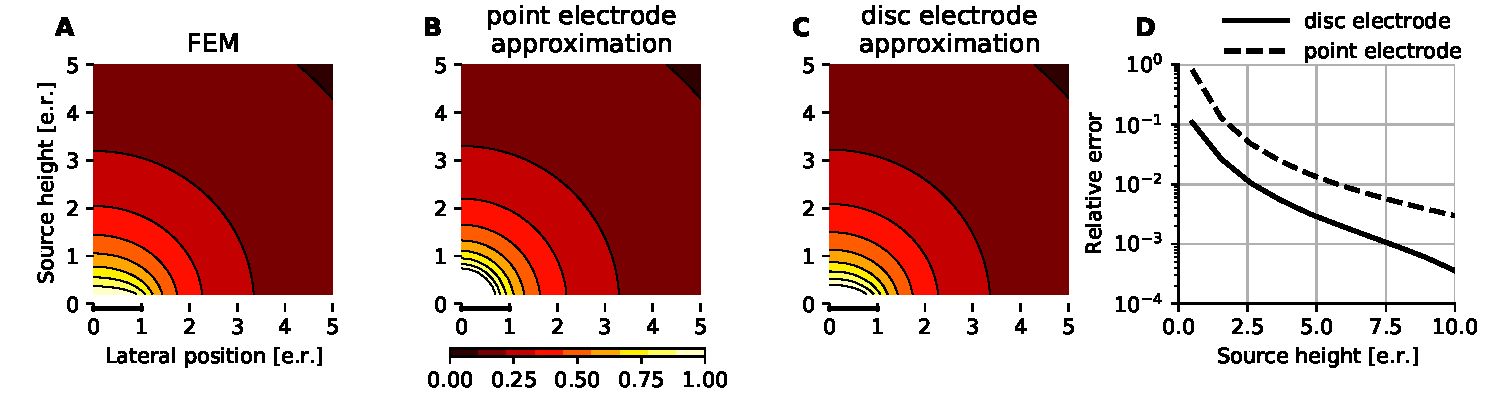
\includegraphics[width=1\textwidth]{Figures/VC/fig_FEM_elec.pdf}
\end{center}
\caption[]{\textbf{Finite Element Method versus the point and disc electrode approximations.}
{\bf A:} The lead-field from an electrode surface at $x$,$y$=0, simulated with the Finite Element Method (FEM). The highly conductive material of the electrode was included in the simulation, as a cylinder protruding out of the bottom of an otherwise homogeneous and isotropic volume conductor. The $x$- and $y$-axes are shown in units of the electrode radius, which in this specific example was 10~\si{\micro\metre}.
{\bf B:} The lead-field from a point current source at the bottom of an homogeneous and isotropic volume conductor, $x$,$y$=0.
{\bf C:} The lead-field from 500 point current source randomly distributed across the electrode surface, centered at $x$,$y$=0. Each current source was scaled by 1/500.
The Method of Images (Sec.~\ref{sec:Sigma:nonhomo}) was used to account for the bottom of the volume for the point- and disc-electrode approximation.
See \citeasnoun**{Ness2015} for full simulation details.
}
\label{fig:VC:FEM_elec}
\end{figure}

In certain cases, like in ECoG \index{ECoG} measurements from the cortical surface, the recording electrodes are both large ($\sim$~2-5~mm diameter) and close to the neuronal sources (the thickness of the human cortex is $\sim$3~mm). In such cases the electrode properties can therefore be expected to have large effect on measured potentials, see for example \citeasnoun**{Vermaas2020b} and \citeasnoun**{Rogers2020}.

\gen{Her maa vi sjekke:} \citeasnoun**{Viswam2019}

\subsection{\blue{Effect of the electrode shanks}}
\label{sec:VC:elec_shafts}
Large multi-contact electrode shanks can be expected to have a substantial effect on close-by extracellular potentials, since it represents a large non-conducting volume \cite**{Moffitt2005,Lempka2011,Mechler2012,Buccino2019}. It has been demonstrated that such large probes can amplify or dampen recorded potentials from nearby cells by almost a factor of two, depending on whether the cell was in front of or behind the electrode shank \cite**{Moffitt2005,Buccino2019}, while no such effects were found for small microwires \cite**{Buccino2019}.
\tvnnote{Can also hurt the brain to push large objects into it, with cell-death, eudema and encapsulation (Moffitt and McIntyre, 2005).}
%%%%%%



\section{\blue{Approximations used in VC theory}}
\label{sec:VC:approximations}

%%%%%%%%%%%%%%%%%%%%%%%%%%%%%%%%
The VC theory presented in this chapter relies on several assumptions and approximations. Firstly, the theory is based on the quasi-static approximation of Maxwell's equations (see \fref{sec:VC:quasistatic} for more on this). Secondly, the the extracellular medium is assumed to be linear, so that the current density is proportional to the electrical field (see \fref{sec:VC:LinEx} for more on this). Thirdly, extracellular currents are assumed to be exclusively due to Ohmic drift, although other currents could in principle be present (see \fref{sec:VC:onlyohmic} for more on this). Fourthly, when applying VC theory, one typically assumes that there is no (ephaptic) feedback from extracellular potentials on the neural activity (see \fref{sec:VC:ephaptic} for more on this). Finally, the extracellular conductivity was throughout this chapter assumed to be isotropic, homogeneous and frequency independent, but it is possible to relax these assumptions. Given its important role, we have devoted an entire chapter of this book to the extracellular conductivity (\fref{chap:Sigma}), where we discuss how the VC theory can be applied also to cases with an anisotropic medium and non-homogeneous medium.


\section{\red{Validation of framework}}
\tvnnote{Jeg foeler vi typisk skriver "extracellular potentials can be modelled by well-established VC theory", og sleger paa en sitering til en kilde som vel egentlig bare sier akkurat det samme.
 Jeg har lyst til aa dedikere litt plass til
"validering". Type: Hvilke beviser finnes for at ECP kan modelleres med transmembrane stroemmer fra kabel-ligning kombinert med VC?
}
